% Relatório do laboratório 3 de servo
% Felipe Bandeira da Silva
% 09/06/2013

%\documentclass[a4paper, 10pt]{article}
\documentclass[paper=a4, fontsize=11pt]{article}

\usepackage[framed,numbered,autolinebreaks,useliterate]{mcode}

\usepackage[brazil]{babel}
\usepackage[utf8]{inputenc}
\usepackage{listings}
\usepackage{color}
\usepackage{amsthm}
\usepackage{graphicx}

\setlength{\parindent}{0pt}
\setlength{\parskip}{18pt}

\title{Relatório, Laboratório 4.\\Servo 1}
\author{Felipe Bandeira da Silva}


%%%%%%%%%%%%%%%%%%%%%%%%%%%%%%%%%%%%%%%%%%%%%%%%%%%%%%%%%%%%%%%%%%%%%%%%%%%%%%%%
% MAIN
%%%%%%%%%%%%%%%%%%%%%%%%%%%%%%%%%%%%%%%%%%%%%%%%%%%%%%%%%%%%%%%%%%%%%%%%%%%%%%%%

\begin{document}

\maketitle

\begin{abstract}
Utilizar o Matlab para analisar a resposta transitória de sistemas de 1ª ordem
ao degrau e estudar o efeito do controle proporcional sobre os aspectos de
estabilidade, velocidade de resposta e erro em regime permanente.
\end{abstract}


\newpage

%%%%%%%%%%%%%%%%%%%%%%%%%%%%%%%%%%%%%%%%%%%%%%%%%%%%%%%%%%%%%%%%%%%%%%%%%%%%%%%
% QUESTÃO 1
%%%%%%%%%%%%%%%%%%%%%%%%%%%%%%%%%%%%%%%%%%%%%%%%%%%%%%%%%%%%%%%%%%%%%%%%%%%%%%%
\section{Primeira questão}

O primeiro sistema fisico é modelado com a equação 1
\begin{equation}
    G_1(s) = \frac{1}{s+1}
\end{equation}

A equação temporal da equação 1 quando submetida a um degrau unitário
é facilmente encontrada aplicando a transformada inversa de laplace,

\begin{equation}
    G_1(s) = \frac{1}{s+1} \frac{1}{s}
\end{equation}

Aplicando o comando $residue$ em 2 para a expansão em frações parciais,

\begin{equation}
    G_1(s) = \frac{-1}{s+1} + \frac{1}{s}
\end{equation}

De 3 é possível encontrar a reposta temporal,

\begin{equation}
    g_1(t) = -e^{-t} + 1
\end{equation}

A plotagem do gráfico pode ser usada para a facilitar o visualização
do comportamento da função,

\begin{center}
    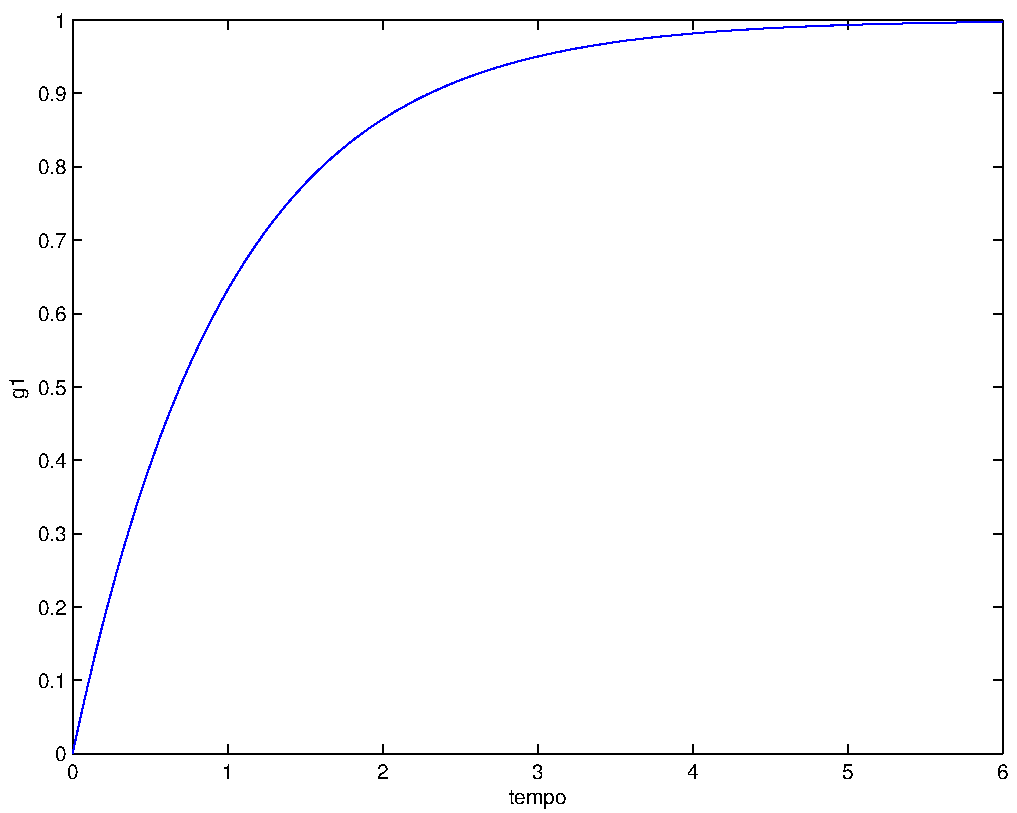
\includegraphics[scale=.39]{q1g1.pdf}
\end{center}

Por inspeção é possível notar que o sistema se estabiliza após um tempo
e seu valor em regimente permanente é 1. Mostrando que o sistema apresenta
uma estabilidade. Esta estabilidade pode ser melhor analisada plotando
a localização dos polos no plano-s.

\begin{center}
    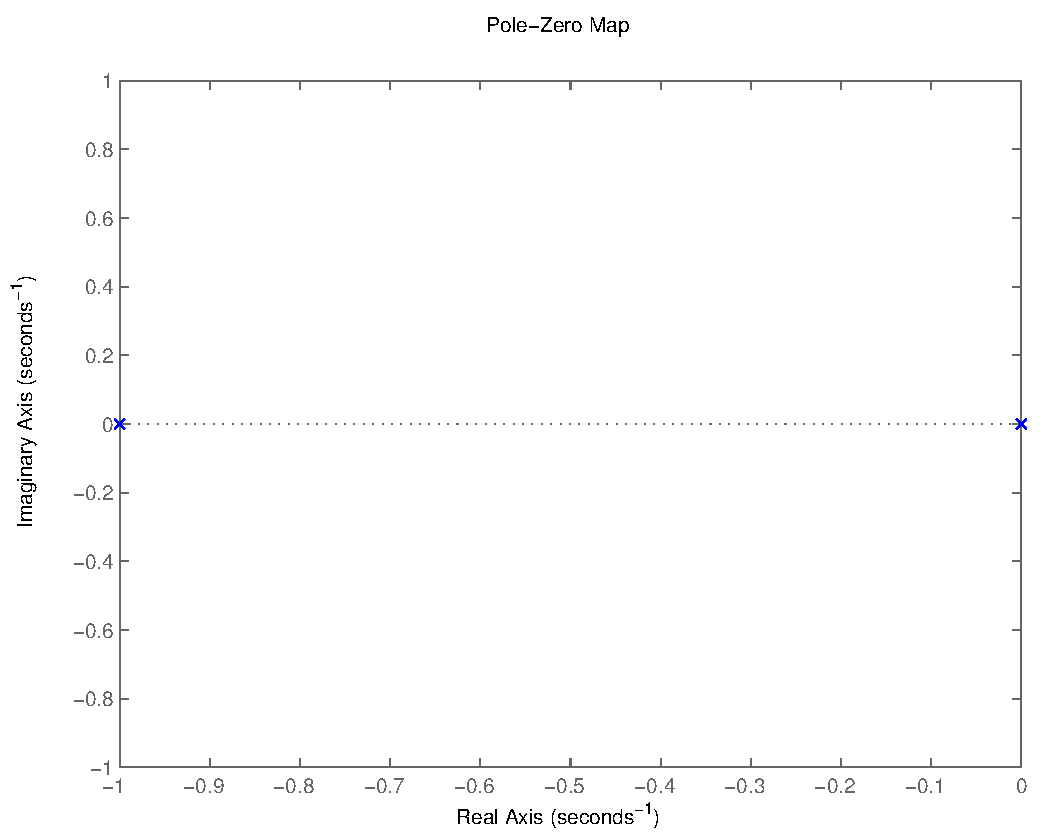
\includegraphics[scale=.5]{pzq1g1.pdf}
\end{center}

Como é possivel observar existem dois polos no eixo real e com valores 
menor igual a zero, mostrando que o sistema é \textbf{estável}.


\end{document}
